\documentclass[12pt]{article}
 
\newenvironment{sol}[1][Solution]{\begin{trivlist}\item[\hskip\labelsep {\bfseries #1:}]}{\end{trivlist}}
\usepackage{minted}
%\usemintedstyle{perldoc}
\usemintedstyle{vs}
\usepackage{graphicx}
\graphicspath{./}

\usepackage[margin=1in]{geometry} 
\usepackage{amsmath,amsthm,amssymb}
\usepackage{times,url}
\usepackage{tikz}
\usepackage{color}
\usepackage{enumerate}
\begin{document}
\renewcommand{\qedsymbol}{\filledbox}
\begin{center}
    \textbf{CS 5/7350 - Test\#2} \\
    \textbf{November 3, 2021}
%replace X with the appropriate number
\end{center}
\begin{flushright}
Name: \underline{Bingying Liang }\\
ID:  \underline{\ \ \ \ \ 48999397 \ \ \ \ \ }
\end{flushright}
\begin{enumerate}
    \item \ [9 pts] Define the following terms as succinctly as possible:
    \begin{itemize}
        \item NP-Hard
        \begin{sol}
                        In computational complexity theory, NP-hardness (non-deterministic polynomial-time hardness) is the defining property of a class of problems that are informally "at least as hard as the hardest problems in `NP". A simple example of an NP-hard problem is the subset sum problem.
        \end{sol}
        \item GCD
                \begin{sol}
            In mathematics, the greatest common divisor (GCD) of two or more integers, which are not all zero, is the largest positive integer that divides each of the integers. For two integers x, y, the greatest common divisor of x and y is denoted $gcd(x,y)$. For example, the GCD of 8 and 12 is 4, that is $gcd(8,14) = 4$.
        \end{sol}
        \item Dynamic Programming
        \begin{sol}
             A dynamic-programming algorithm solves each subsubproblem just once and then saves its answer in a table, thereby avoiding the work of recomputing the answer every time it solves each subsubproblem. 
        \end{sol}
        \item Longest Common Subsequence
        \begin{sol}
             Given two sequences X and Y, we say that a sequnence Z is common subsequence of X and Y if Z is a subsequence of both X and Y. For example, if X = \{A,B,C,D,A,B\} and Y =\{B, D, C, A, B, A\}, the sequence \{B,C,A\} is a common subsequence of both X and Y. The sequence\{B,C,A\} is not a longest common subsequence (LCS) of X and Y, however, since it has length 3 and the sequence \{B, C, B, A\}, which is also common to both sequences X and Y, has length 4. The sequence \{B, C, B, A\} is an LCS of X and Y, as is the sequence \{B, C, A, B\}, since X and Y have no common subsequence of length 5 or greater.
        \end{sol}
        \item Heap
        \begin{sol}
            In computer science, a heap is a specialized tree-based data structure which is essentially an almost complete binary tree that satisfies the heap property: in a max heap, for any given node C, if P is a parent node of C, then the key (the value) of P is greater than or equal to the key of C. In a min heap, the key of P is less than or equal to the key of C. The node at the "top" of the heap (with no parents) is called the root node.
        \end{sol}
        \item LZW
        \begin{sol}
            Lempel–Ziv–Welch (LZW) is a universal lossless data compression algorithm created by Abraham Lempel, Jacob Ziv, and Terry Welch. It was published by Welch in 1984 as an improved implementation of the LZ78 algorithm published by Lempel and Ziv in 1978. The algorithm is simple to implement and has the potential for very high throughput in hardware implementations. It is the algorithm of the Unix file compression utility compress and is used in the GIF image format.
        \end{sol}
    \end{itemize}

    \item \ [2 pts] Compute $\Phi(55)=$
    \begin{sol}
        $\Phi(55)=\Phi(5 \times 11) = (5-1)\times (11-1) = 4 \times 10 = 40$
    \end{sol}

    \item \ [6 pts] If a smallest last ordering has the largest degree when deleted of 9 and a terminal clique size of 8
    \begin{enumerate}
        \item What is the maximum number of colors that might be required by the ordering?
        \begin{sol}
        10
        \end{sol}
        \item What is the minimum number of colors that must be required by the graph?
        \begin{sol}
            8
        \end{sol}
    \end{enumerate}

    \item \ [9 pts] Consider the Smallest Last Vertex Ordering:
    \begin{enumerate}
        \item Draw a graph and give a smallest last vertex ordering of that graph where
the terminal clique is not the largest complete subgraph in the graph. (Note the terminal clique is the complete subgraph at the end of deleting vertices with the SLVO algorithm)
    \begin{sol}
    \hspace*{\fill}
                    \begin{center}
        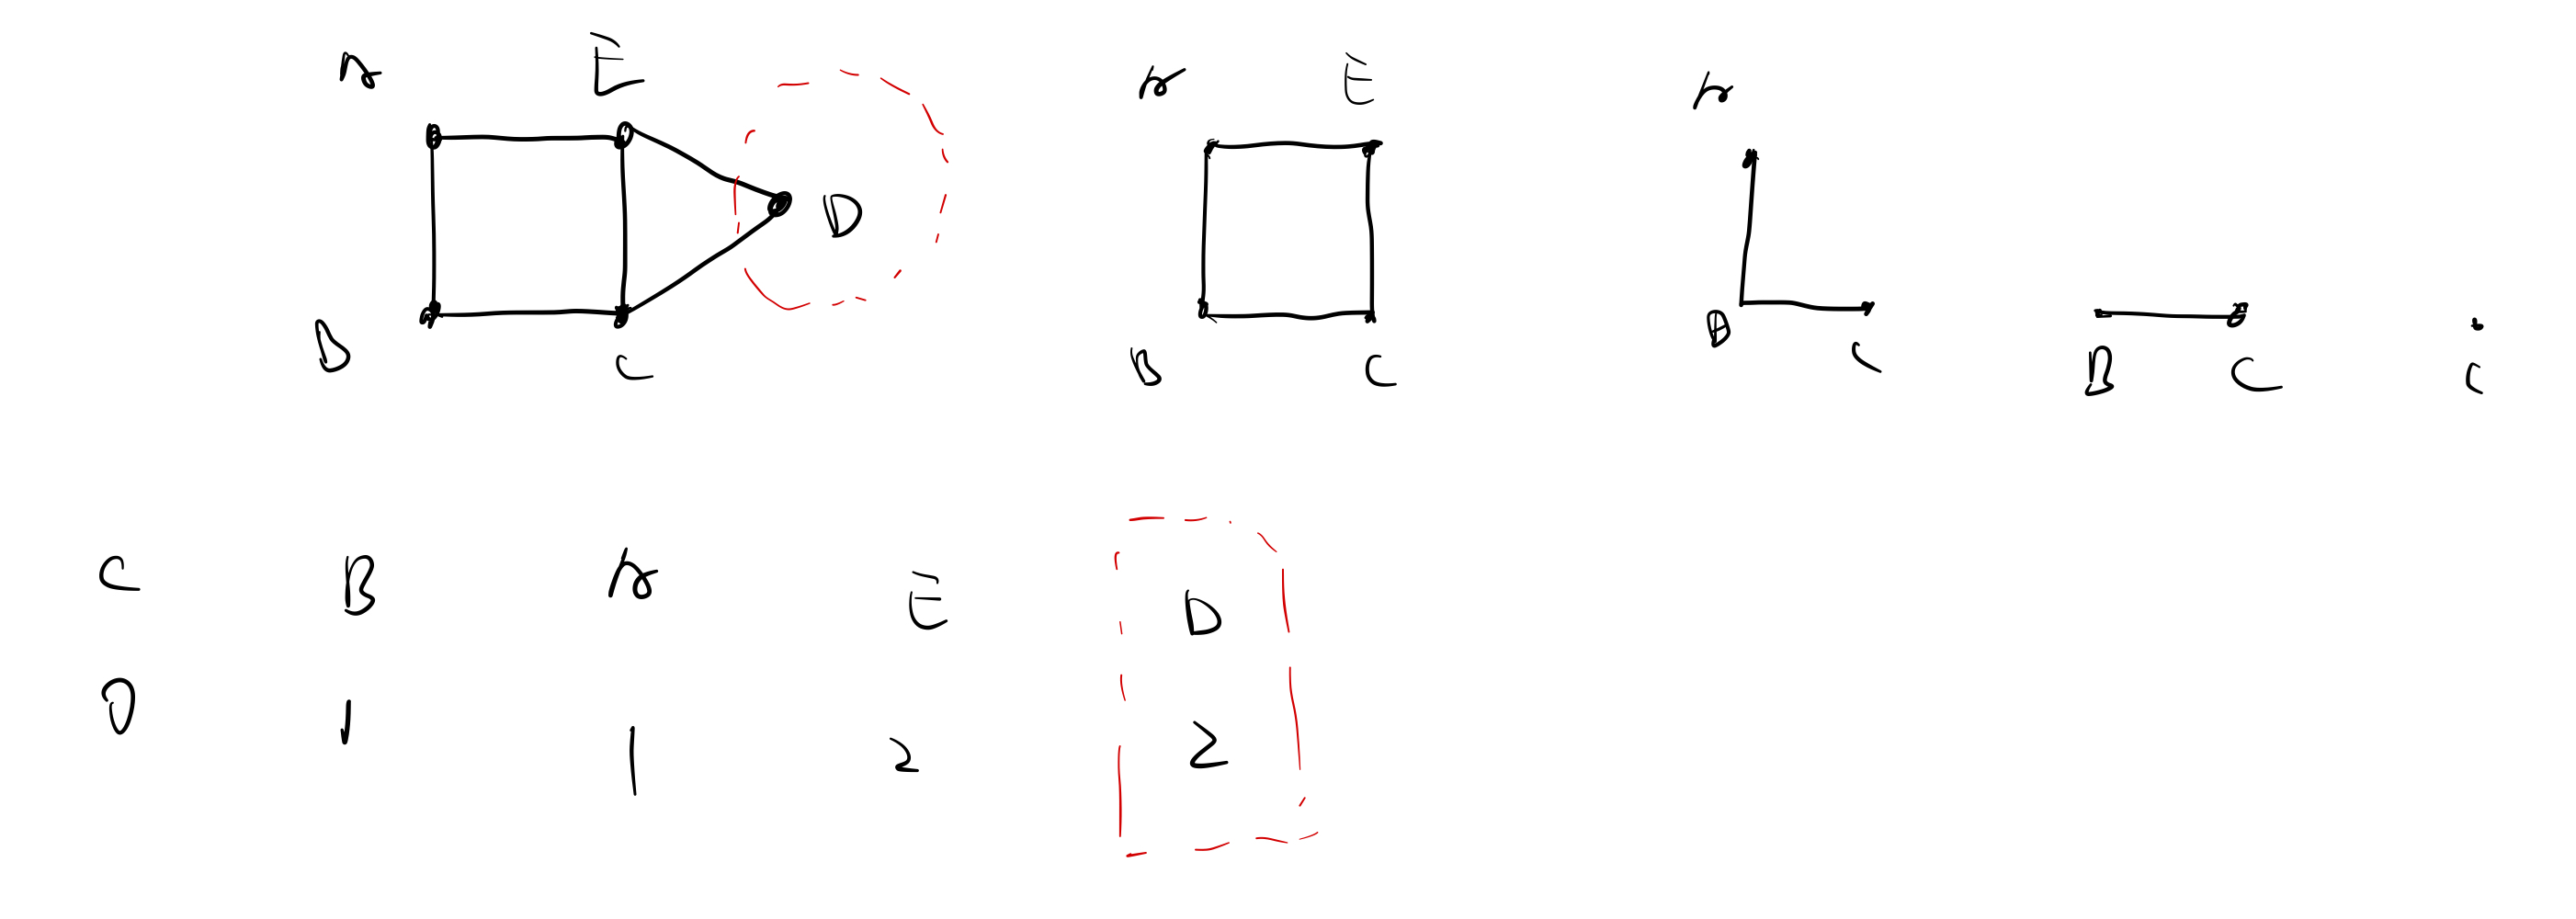
\includegraphics[width=0.9\textwidth]{p2.jpeg}
    \end{center}
    \end{sol}
    
\item Give another smallest last vertex ordering for the graph above where the terminal clique is the largest complete subgraph in the graph.
    \begin{sol}
    \hspace*{\fill}
                    \begin{center}
        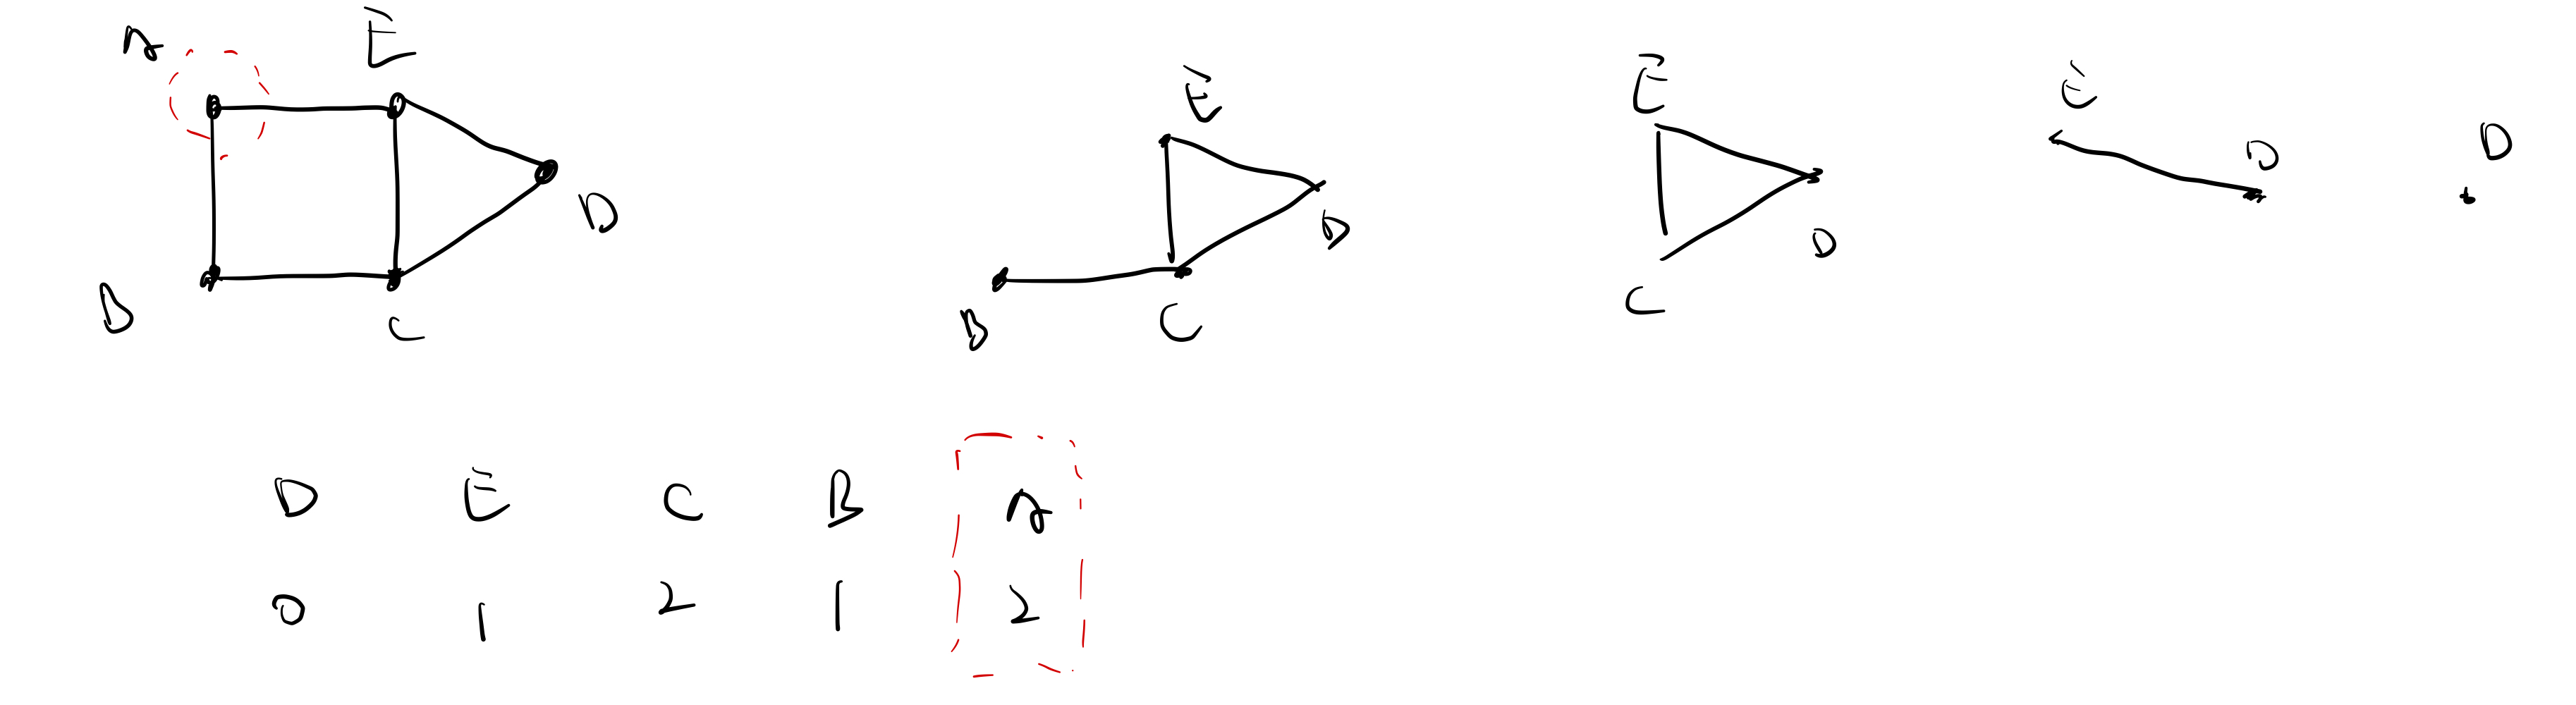
\includegraphics[width=0.9\textwidth]{p3.jpeg}
    \end{center}
    \end{sol}
    \end{enumerate}


    \item \ [12 pts] Consider the following NP completeness questions. Answer them with “some” “all” “none” or “unknown”
    \begin{enumerate}
        \item Which Problems in P are also in NP? (“some” “all” “none” or “unknown”)
        \item Which Problems in NP-Hard are also in NP? ( “some” “all” “none” or “unknown”)
        \item Which Problems in NP-Complete are in NP-Hard ( “some” “all” “none” or “unknown”)
        \item If someone can solve an NP-Hard problem in Polynomial Time, then all NP and all NP complete problems can be solved in polynomial time. (true or false)
        \item At least 1 NP problem can be solved in polynomial time? (True or False)
        \item NP-Complete problems are in P (“true” “false” or “unknown”)
        \item At least 1 NP problem can be solved in polynomial time? (True or False)
        \item Which NP-Hard Problems are also NP-Complete? ( “some” “all” “none” or “unknown”)
    
    \end{enumerate}
    \item \ [8 pts] Consider a Heap:
    \begin{enumerate}
        \item How many swaps in the worst case may be required to form a heap
using the HEAPIFY algorithm from an array of 21 items?
\begin{sol}
7+6+5=18
\end{sol}
\item How many swaps in the worst case may be required for inserting an item into a heap with 21 items before the insert.
\begin{sol}
    4
\end{sol}
    \end{enumerate}

    \item \ [9 pts] Consider an RSA encryption system that has a public key of 8591 for the value e and 95129 for the value of the modulus N. You also saw a message that had been encrypted by the public key. The value of this encrypted message is 18407.
    \begin{enumerate}
        \item You are able to factor N=95129 into the product of two prime numbers 379 * 251. What is the value of the private key? Show your work including the table for computing the Extended Euclidean Algorithm.
                \begin{sol}
        \hspace*{\fill} \\
        public key: (e,n) = (8591, 95129)\\
        private key: (d,n)
        \begin{align*}
            &d = \frac{1}{e}\bmod \Phi(n) = \frac{1}{8591} \bmod \Phi(95129)\\
            &\Phi(95129)= \Phi(379 \times 251)=(379-1)\times(251-1)=378 \times 250 = 94500 \\
            &\therefore d = \frac{1}{8591} \bmod 94500
        \end{align*}
            \begin{center}
                \begin{tabular}{|c|c|c|c|c|c|c|}
                \hline
                     & A & B&Q &R &$\alpha$ & $\beta$  \\ 
                     \hline
                                       -1 &  & & & & 1 & 0 \\ 
                     \hline
                        & 94500 & 8591 & 10 & 8590 & 0 & 1 \\ 
                     \hline
                           &  8591 & 8590& 1 & 1  & 1& -10 \\ 
                     \hline
                               &  8590 &1 &8590 &0 & -1&  11  \\      
                     \hline
                                    & 1 &0 &- &- & 8591& -94500 \\ 
                     \hline

                \end{tabular}
            \end{center}
            \begin{align*}
                &(-1) \times(94500)  + 11 \times 8591 = 1\\
                &(-94500) \bmod 95129 +(11\times 8591)\bmod 95129 = 1\\
                & (11 \times 8591) \bmod 95129 = 1\\
                & \because (\frac{1}{8591} \times 8591) \bmod 95129 = 1 \\
                & \therefore d = \frac{1}{8591}\bmod 95129 = 11 \\
                & \therefore \text{private key:} (11, 95129)
            \end{align*}
        \end{sol}
        \item What was the message before it was encrypted (you may give a formula)
        \begin{sol}
        \begin{align*}
            (18407)^{11} \bmod 95129 = 17
        \end{align*}
        \end{sol}
    \end{enumerate}
    
    \item \ [7 pts] A sequence of 21 values was used with the Longest Increasing Subsequence algorithm to create the following table (the 99’s are equivalent to infinity). The actual values in the original sequence have been omitted from the table:
            \begin{center}
        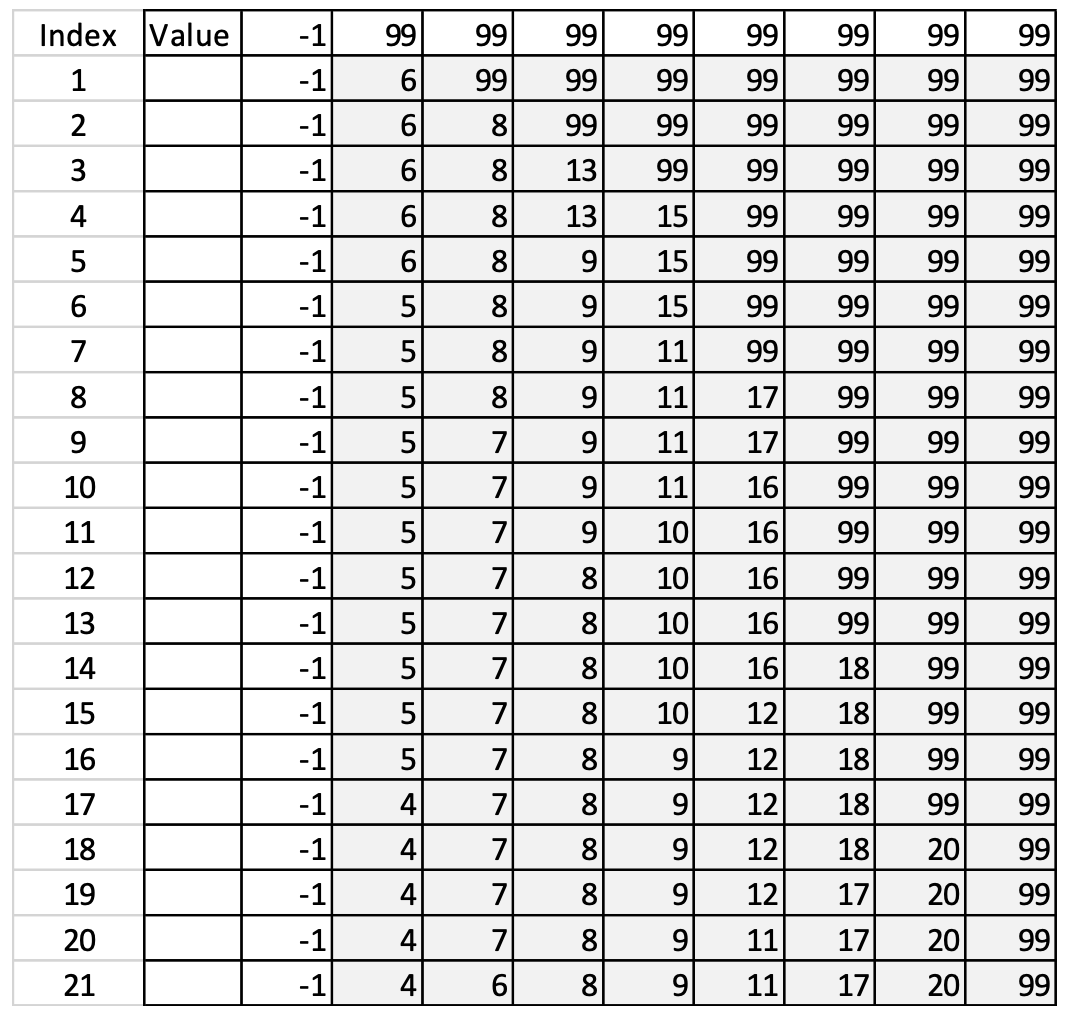
\includegraphics[width=0.9\textwidth]{1.png}
    \end{center}


    \begin{enumerate}
        \item What is the longest increasing subsequence of the original sequence?
        \begin{sol}
        6, 8, 9, 11, 16, 18, 20
        \end{sol}
        \item \textcolor{red}{What does the value 11 represent on the last row?}
        \begin{sol}
            11 is the smallest ending value of a subsequence of lengths.
        \end{sol}
    \end{enumerate}

    \item \ [9 pts] Consider the Levensthein Edit Distance for two strings A and B.
    \begin{enumerate}
        \item Write the equation describing what you would put in the table for location T[i,j].
        \begin{sol}
        \hspace*{\fill}
        \begin{minted}[frame=lines,framesep=2mm,baselinestretch=1.2,fontsize=\footnotesize,linenos]{c}
// base case
if (i == 0){
    T[i,j] = T[0, j];
}
if (j == 0){
    T[i,j] = T[i, 0];
}
if (Ai == Bj){
    T[i,j] = min{T[i-1,j]+1,T[i, j-1]+1, T[i-1,j-1]};
}else{
    T[i,j] = min{T[i-1,j]+1, T[i,j-1]+1,T[i-1,j-1]+1};
}
        \end{minted}
        \end{sol}
        \item How would you modify this equation for a different version of the Levensthein Edit Distance where substitution is not allowed?
                \begin{sol}
        \hspace*{\fill}
        \begin{minted}[frame=lines,framesep=2mm,baselinestretch=1.2,fontsize=\footnotesize,linenos]{c}
if (Ai == Bj){
    T[i,j] = min{[i-1,j]+1,[i, j-1]+1, [i-1,j-1]};
}else{
    T[i,j] = min{[i-1,j]+1, [i,j-1]+1,[i-1,j-1]+1};
}
        \end{minted}
        \end{sol}
        \item Fill in the following table for finding the regular, unmodified “Levensthein Edit Distance” for two strings, M and N
        \begin{center}
            M \ = \ A \ X \ B \ Y \ C \ \ \ \ \ N \ = \ A \ Z \ B \ C \ Y
        \end{center}

        \begin{sol}
        \hspace*{\fill}
        \begin{center}
            \begin{tabular}{|c|c|c|c|c|c|c|}
            \hline
                  &- & A & X & B & Y & C  \\
                  \hline
                 - &0 & 1& 2 &3 & 4& 5\\
                 \hline
                A & 1 & 0  & 1  & 2  & 3  &4 \\
                \hline
                Z &  2 & 1  & 1  &2   & 3  & 4\\
                \hline
                B &  3 &  2  & 2  & 1  & 2  &3 \\
                \hline
                C &  4 &  3 & 3  & 2  & 2  &3 \\
                \hline
                Y &  5 &  4 & 4  & 3  & 2  &3 \\
                \hline
            \end{tabular}
        \end{center}
        \end{sol}


    \end{enumerate}

    \item \ [8 pts] You know that problem B is NP-Complete and you want to use that to prove that problem A is NP-Complete. What two things must you show about problem A?
    \item \ [12 pts] You have 4 dice. Each one is different. Die \#1 has sides \{ -1, 0, 1 \}. Die \#2 has sides \{ -1, -1, 0, 0 \} Die \#3 has sides \{1, 1, 1, 1\} and Die \#4 has sides \{0,0,0, 1,1,1\}
    \begin{enumerate}
        \item Fill in the table below
         \begin{sol}
        \hspace*{\fill}
        \begin{center}
            \begin{tabular}{|c|c|c|c|c|}
            \hline
                 & Die\#1 & Die \#1,\#2 & Die \#1, \#2, \#3 & Die \#1,\#2,\#3,\#4  \\
                \hline
                -2 & 0 &2 & 0& 0 \\
                \hline
                -1 & 1 &4 ,  & 8& 24 \\
                \hline
                0&  1 &4 & 16& 72 \\
                \hline
                1&  1 &2 & 16 & 96 \\
                \hline
                2&  0 &0 & 8& 72 \\
                \hline
                3&  0 &0 & 0& 24 \\
                \hline
                4 & 0 &0 & 0& 0 \\
                \hline
                Sum& 3 &12 & 48& 288 \\
                \hline
            \end{tabular}
        \end{center}
        \end{sol}
        \item How many ways can you roll a 0 with these 4 dice?
        \begin{sol}
            72
        \end{sol}
        \item What is the probability of rolling a 0 with these 4 dice?
                \begin{sol}
            $\frac{1}{4}$
        \end{sol}
        \item How many ways can you roll a 2 with these 4 dice?
                \begin{sol}
            72
        \end{sol}
        \item What is the probability of rolling a 2 with these 4 dice?
        \begin{sol}
            $\frac{1}{4}$
        \end{sol}
    \end{enumerate}

    \item \ [9 pts] You have received a message that was compressed with LZW. Remember that A=65, B=66, C=67, D=68 and E=69. The dictionary starts with entry 256. The message you received was
    \begin{align*}
        67  \ 65 \ 67 \ 68  \ 257 \ 256  \ 69 \ 258 \ 260
    \end{align*}
    \begin{enumerate}
        \item What was the original message and what is your dictionary after decompression?
                 \begin{sol}
        \hspace*{\fill}\\
        \begin{center}
        \begin{tabular}{|c|c|}
        \hline
             Dictionary  \\
             \hline 
             A = 65 \\
             \hline
             B = 66 \\
             \hline 
             C = 67 \\
             \hline 
             D = 68 \\
             \hline 
             E = 69 \\
             \hline 
             ...\\
             \hline
             256 = CA \\
             \hline 
             257 = AC \\
             \hline 
             258 = CD \\
             \hline 
             259 = DA \\
             \hline
             260 = ACC \\
             \hline 
             261 = CAE \\
             \hline 
             262 = EC \\ 
             \hline
             263 = CDA\\
             \hline
        \end{tabular}
        \\
        \begin{tabular}{|c|c|c|c|c|c|c|}
        \hline
            &start \ $w$ & read $k$ & entry & output & Dictionary add & next \ $w$  \\
            \hline
             0& - & 67 & C & C & &  C  \\
             \hline 
            1&  C & 65 & A & A & CA = 256 & A \\ 
            \hline 
            2&  A & 67 & C & C &AC = 257 & C \\
            \hline
             3&  C & 68 & D & D &CD = 258 & D \\ 
             \hline
            4& D & 257 & AC & AC &DA = 259 & AC \\
            \hline
             5& AC & 256 &CA & CA & ACC = 260 & CA \\ 
             \hline
            6& CA & 69 & E & E &  CAE = 261 & E \\
            \hline
             7&  E & 258 & CD &CD & EC = 262 & CD   \\ 
             \hline
            8& CD &  260 & ACC & ACC & CDA = 263 & ACC \\
            \hline
             9&  &  &  & & & \\ 
             \hline

        \end{tabular}
                \end{center}
        The original message is: C, A, C, D, AC, CA, E, CD, ACC.
        \end{sol}
        \item Assuming 8 bits per character, how many bits were in the uncompressed message?
        \begin{sol}

                \begin{align*}
                    8 \times 14 = 112 \ bits
                \end{align*}

        \end{sol}
        \item Assuming the last entry of your dictionary was 2047, how many bits were in the compressed message
               \begin{sol}

                \begin{align*}
                    & \log_2{2047+1} = \log_2{2048} = 11\\
                    & 11 \times 9 = 99 \ bits
                \end{align*}

        \end{sol}
    \end{enumerate}
 

\end{enumerate}


\end{document}
